% begin module polar-curve-ex8
\begin{frame}
\begin{example}[Example 8, p. 679]
Sketch the curve $r = \cos 2\theta$.
\begin{columns}[c]
\column{.3\textwidth}
\ \only<handout:0| 1>{%
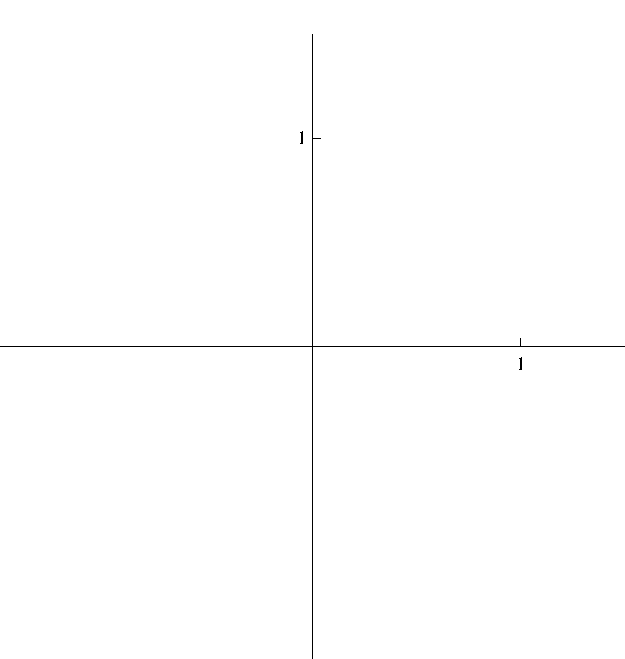
\includegraphics[height=3.6cm]{polar-curves/pictures/11-03-ex8a.pdf}%
}%
\only<handout:0| 2>{%
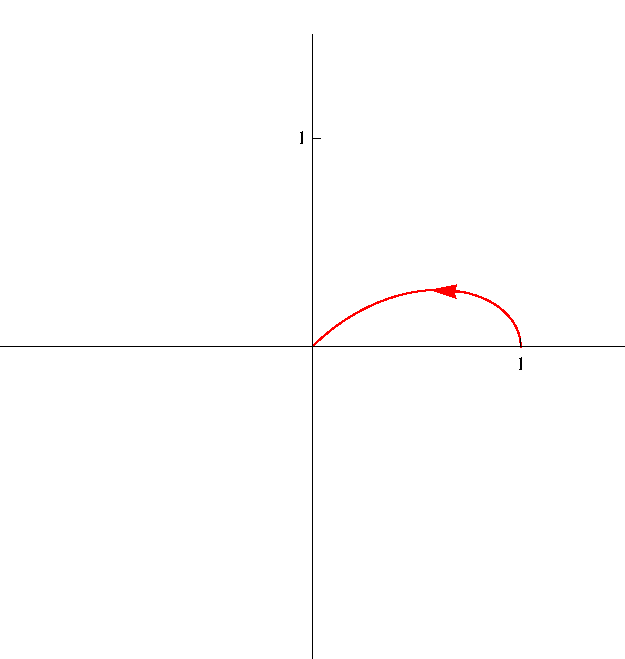
\includegraphics[height=3.6cm]{polar-curves/pictures/11-03-ex8b.pdf}%
}%
\only<handout:0| 3>{%
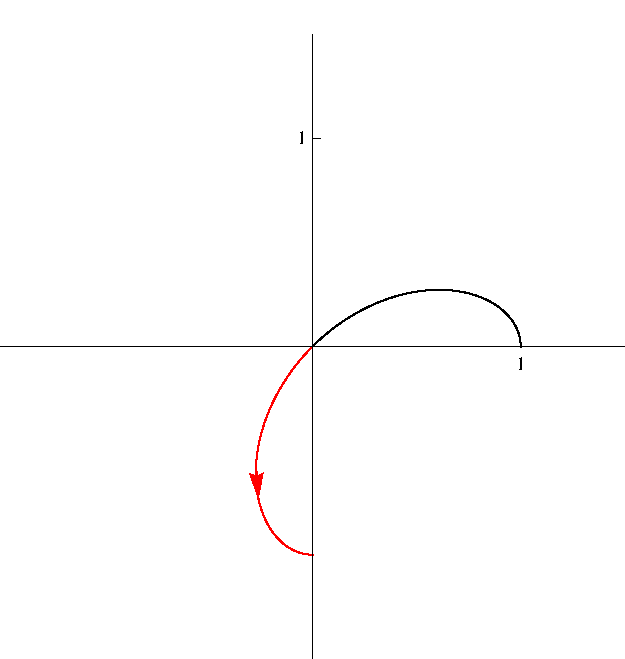
\includegraphics[height=3.6cm]{polar-curves/pictures/11-03-ex8c.pdf}%
}%
\only<handout:0| 4>{%
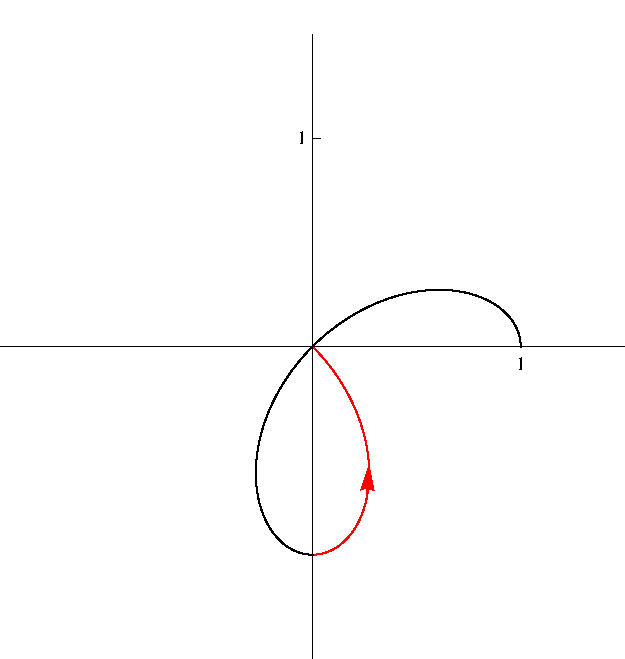
\includegraphics[height=3.6cm]{polar-curves/pictures/11-03-ex8d.pdf}%
}%
\only<handout:0| 5>{%
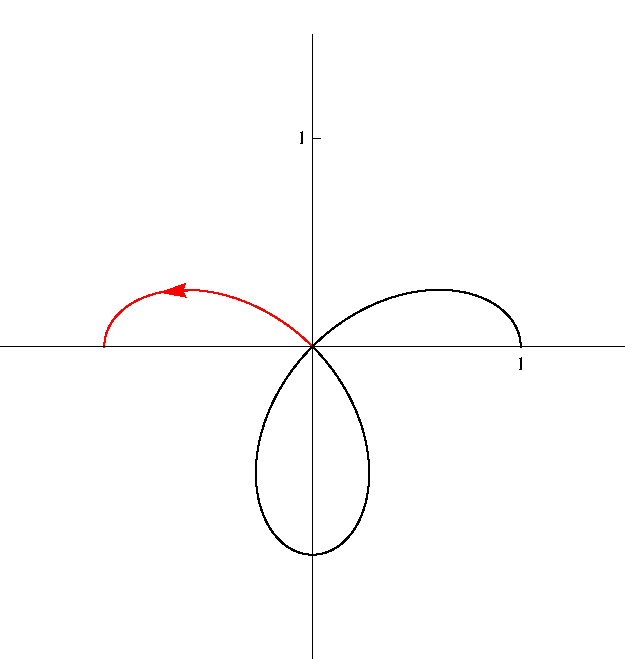
\includegraphics[height=3.6cm]{polar-curves/pictures/11-03-ex8e.pdf}%
}%
\only<handout:0| 6>{%
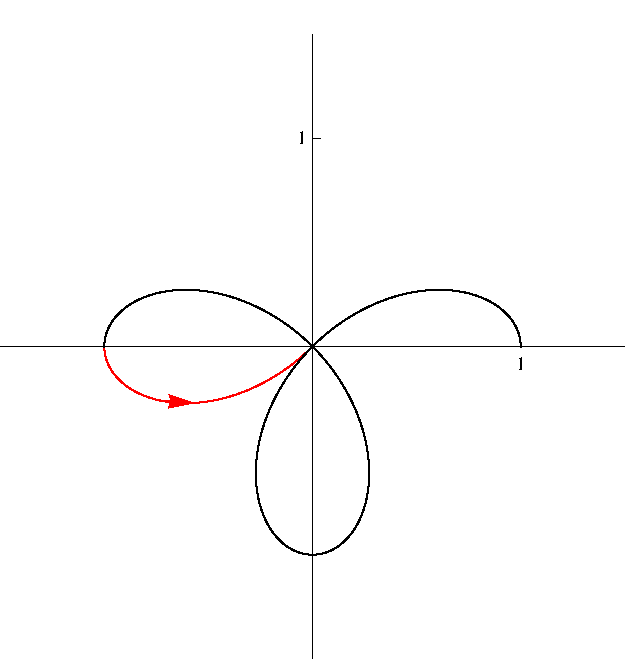
\includegraphics[height=3.6cm]{polar-curves/pictures/11-03-ex8f.pdf}%
}%
\only<handout:0| 7>{%
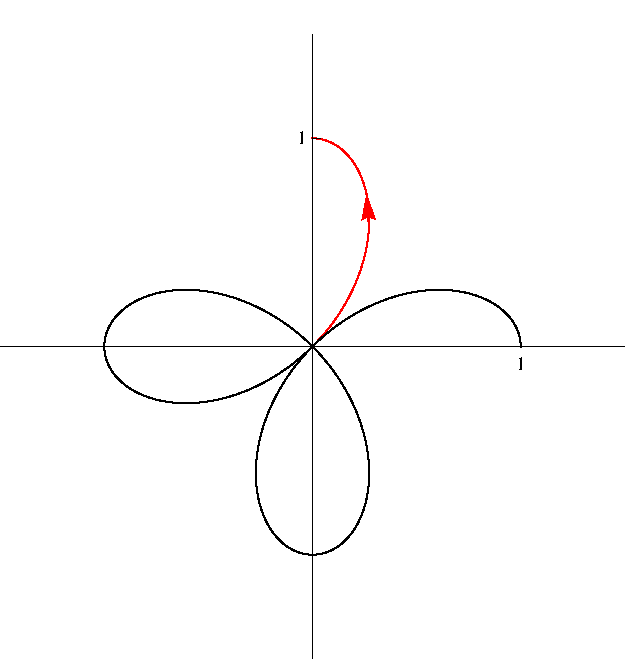
\includegraphics[height=3.6cm]{polar-curves/pictures/11-03-ex8g.pdf}%
}%
\only<handout:0| 8>{%
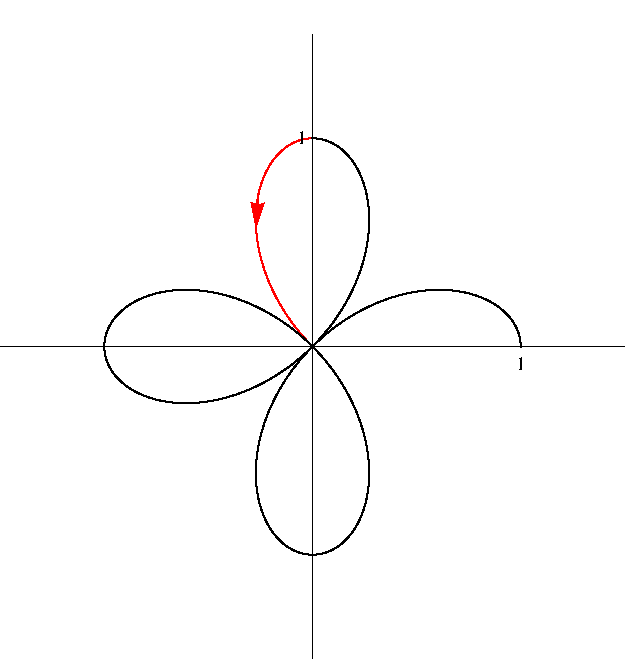
\includegraphics[height=3.6cm]{polar-curves/pictures/11-03-ex8h.pdf}%
}%
\only<9->{%
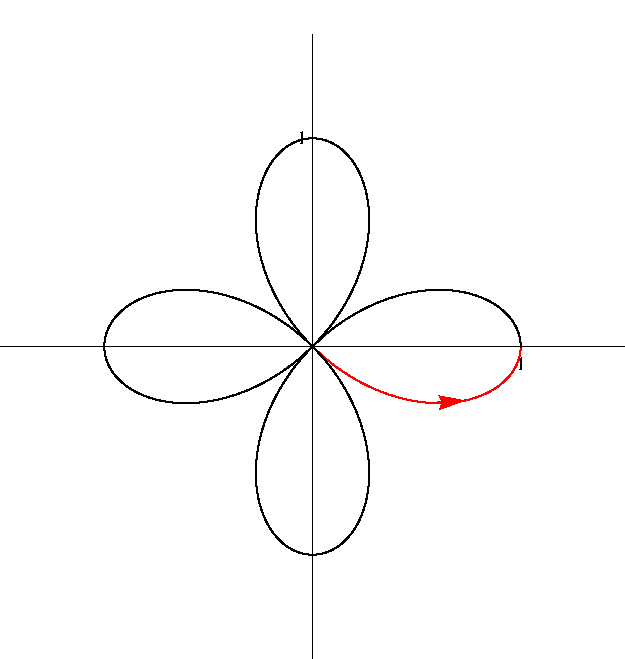
\includegraphics[height=3.6cm]{polar-curves/pictures/11-03-ex8i.pdf}%
}%
\column{.7\textwidth}
\ \only<handout:0| 1>{%
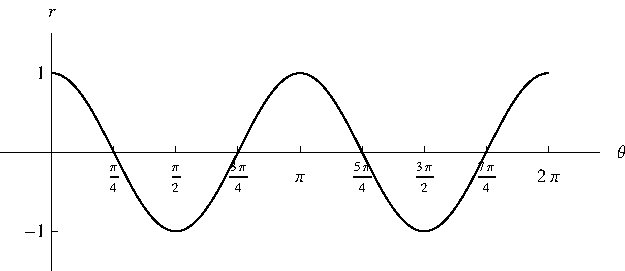
\includegraphics[height=3.6cm]{polar-curves/pictures/11-03-ex8helpera.pdf}%
}%
\only<handout:0| 2>{%
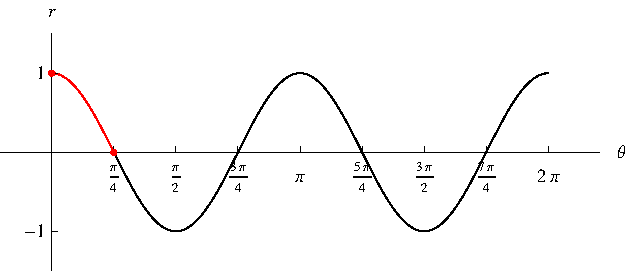
\includegraphics[height=3.6cm]{polar-curves/pictures/11-03-ex8helperb.pdf}%
}%
\only<handout:0| 3>{%
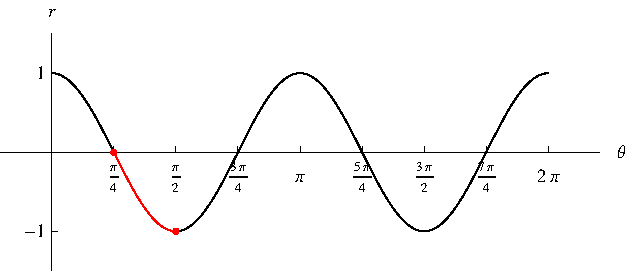
\includegraphics[height=3.6cm]{polar-curves/pictures/11-03-ex8helperc.pdf}%
}%
\only<handout:0| 4>{%
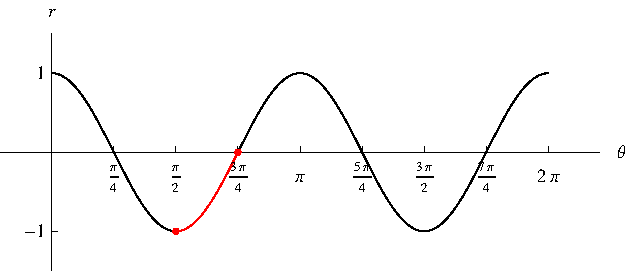
\includegraphics[height=3.6cm]{polar-curves/pictures/11-03-ex8helperd.pdf}%
}%
\only<handout:0| 5>{%
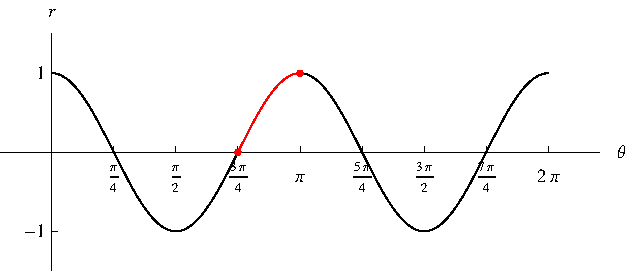
\includegraphics[height=3.6cm]{polar-curves/pictures/11-03-ex8helpere.pdf}%
}%
\only<handout:0| 6>{%
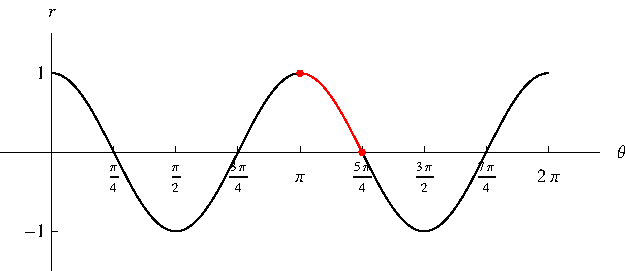
\includegraphics[height=3.6cm]{polar-curves/pictures/11-03-ex8helperf.pdf}%
}%
\only<handout:0| 7>{%
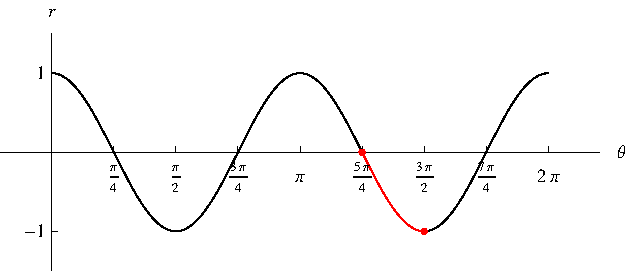
\includegraphics[height=3.6cm]{polar-curves/pictures/11-03-ex8helperg.pdf}%
}%
\only<handout:0| 8>{%
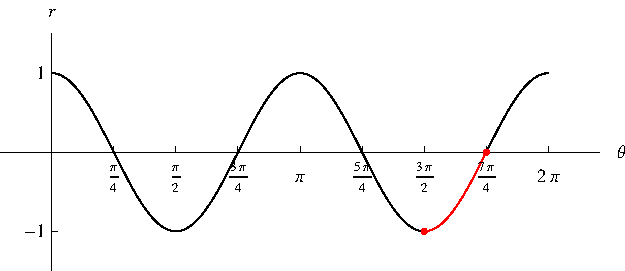
\includegraphics[height=3.6cm]{polar-curves/pictures/11-03-ex8helperh.pdf}%
}%
\only<9->{%
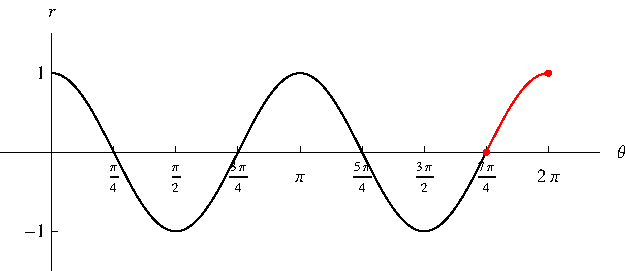
\includegraphics[height=3.6cm]{polar-curves/pictures/11-03-ex8helperi.pdf}%
}%
\end{columns}
\end{example}
\end{frame}
% end module polar-curve-ex8
